% \documentclass[preprint]{kcc}
\documentclass{kcc}


%%%%%%%%%%%%%%%%%%%%%%%%%%%%%%%%%%%%%%%%%%%%%%%
% include additional packages you need to use
%%%%%%%%%%%%%%%%%%%%%%%%%%%%%%%%%%%%%%%%%%%%%%%
% graphic, float package
\usepackage{graphicx}		% for setting images
\usepackage{float}			% for float objects
\usepackage{subfloat}		
\usepackage{subfigure}		% for adding several figures in a figure environment
\usepackage{lscape}			% for landscape type images or tables


\usepackage{enumitem}

% for compact section title spacing
% \usepackage[compact]{titlesec}

% nameref
\usepackage{nameref}

% mathmetical presentation
\usepackage{gensymb}
\usepackage{amsmath}
\usepackage{amssymb}
\usepackage{amsthm}
\usepackage{exscale}
\usepackage{textcomp}		% extra symbols


% for circled number
\newcommand{\cl}[1]{\textcircled{\scriptsize #1}}


% package for using algorithmic presentation
\usepackage{algorithmic}
\usepackage{algorithm}
% customize algorithmic environment
\renewcommand{\algorithmicrequire}{\makebox[40px]{\hfill\textbf{Input :}}}
\renewcommand{\algorithmicensure}{\makebox[40px]{\hfill\textbf{Output :}}}

% array and table presentation
\usepackage{array}
\usepackage{tabulary}
\usepackage{multirow}
\usepackage[table]{xcolor}
\usepackage{ctable}
\usepackage{booktabs}		% for typesetting tables at the level of publication		
							% do not use vertical rule
							
% set title, author, abstract
\title{비디오 시청 환경에서의 장기 기억에 대한 안구 운동 분석}
\author{
김진화$^{\circ1}$, 장병탁$^{1234}$\\
서울대학교 인지과학 협동과정$^{1}$\\
서울대학교 컴퓨터공학부$^{2}$\\
서울대학교 뇌과학 협동과정$^{3}$\\
서울대학교 생물정보학 협동과정$^{4}$\\
\{jhkim, btzhang\}@bi.snu.ac.kr
}
\engtitle{Eye Movement Analysis for Long-term Memory on Video Stimuli}
\engauthor{
Jin-Hwa Kim$^{\circ1}$, Byoung-Tak Zhang$^{1234}$\\
Cognitive Science Program$^{1}$, School of Computer Science and Engineering$^{2}$, \\
Brain Science Program$^{3}$, Bioinformatics Program$^{4}$, Seoul National University\\
}
\abstract{
안구 운동은 뇌 활동을 관찰할 수 있는 비침습적이면서 활용도가 높은 지표이다. 이러한 배경으로 최근 안경류 웨어러블 장비가 연구 기관을 중심으로 빠르게 보급되고 있으며 안구 운동에 대한 연구 활동과 관련 산업의 성장을 고도화 하고 있다. 우리는 아동용 비디오 시청 환경에서 안구 운동을 연구하였다. 우리는 응시 기간에 따른 장기 기억 상관 여부를 확인해 보았지만 유의성을 발견할 수 없었다. 하지만 시청각 자극을 \textit{주의} 상황과 \textit{중립} 상황으로 나눈 후 응시 기간에 따른 차이를 확인하였을 때 긴 응시에서는 장기 기억 인출에서 통계적으로 유의미한 차이를 발견할 수 있었지만 짧은 응시에서는 그렇지 못하였다. 이러한 안구 운동 특징에서 발견되는 장기 기억과 관련된 인지 과정을 계산학적으로 모델링하고 간접적으로 그 효율적인 정보 처리 기제에 대해 논의하였다. 이는 평생 학습 기제에는 선택적 주의를 통한 효율성 추구가 제한된 인지 처리 능력 안에서 중요한 요소로 기여함을 시사한다.
}


\begin{document}

\maketitle


\section{서 론}
안구 운동은 물리적으로 여섯 개의 근육을 이용하여 시선을 움직이고 고정시킨다. 이 여섯 개의 근육은 상하 좌우 및 회전하는 방향으로 각각 두 개의 근육이 수축하고 이완하며 조절한다. 이러한 근육 운동은 자율적으로 또는 무의식적으로 일어나는데 뇌로부터 안구 운동에 이르는 신경 신호 전달 경로는 하나 이상으로 다양한 영역에서 관여한다.

안구 운동 측정기로부터 관찰되는 안구 운동은 크게 세가지로 분류할 수 있다. 첫번째는 한 지점을 바라보는 고정 상태인 응시이다. 응시는 의도적으로 주의를 기울여도 완벽히 한 지점을 바라볼 수 없는데 안구 근육의 수축 또는 이완의 상태를 유지하는 데 분자 수준에서의 지속적인 화학 반응이 필요하기 때문이다. 두번째는 도약 운동이다. 응시와 응시 사이에는 상대적으로 빠른 안구 움직임이 있는데 이를 도약 운동이라고 한다. 응시와 도약 운동을 분리하는 일은 실험의 목적에 따라 특별히 고안된 여과 함수를 통해 수행한다. 가장 많이 사용하는 여과 방법으로는 초당 움직인 각도를 기준으로 응시와 도약 운동을 분류하며 일반적으로 초당 30 도 이상 움직이게 되면 도약 운동으로 분류한다. 세번째는 부드러운 추적 운동이다. 천천히 움직이는 시각 자극을 쫓는 시선 궤적은 초당 30 도 이하의 속력으로 움직이지만 경향성을 가진 시선 이동을 만들어 낸다. 본 논문에서는 부드러운 추적 운동에 대한 분석은 생략하였다.

많은 심리학자들과 신경과학자들에 의해 읽기 환경에서 안구 운동을 연구 하였다 \cite{Rayner1998,Reichle1998}. 특히 통제된 읽기 자료를 이용한 안구 운동 연구\cite{Inhoff1986,Rayner1986}는 단어 빈도 수 등과 같은 언어학적 특징과 응시 기간의 관련성을 보이며 응시 기간을 인지 처리 작업량을 나타내는 지표로 해석하기 시작했다. 

시청 환경에서는 감정을 유발하는 장면이나 내용의 문맥이 장기 응시를 유발할 수 있고 다음 응시를 선택하거나 도약 운동 방향을 결정할 때 단어 배치 분포를 따라 좌우 이동이 우세한 읽기 환경과는 달리 훨씬 자유롭다는 점에서 중요한 차이를 보인다.

따라서 시청 환경에서의 안구 운동 분석은 읽기 환경과 비교할 때 연구의 복잡성 증가와 방법론적 어려움 때문에 충분히 연구되지 못하고 있었다 \cite{Tatler2011}. 하지만 최근에는 구글 글래스와 같은 웨어러블 장비의 개발과 휴대용 안구 운동 측정기의 보급은 보다 자유로운 환경에서의 실험을 가능하게 했고 안구 운동 연구 주제 범위를 넓혔으며 시각 자극의 현저점 분석 기법\cite{itti1998model}은 다양한 응용 기술 개발을 촉진시켰다. 

본 논문에서는 시청 환경에서 안구 운동을 장기 기억 형성과 관련하여 분석하였다. 안구 운동을 응시와 도약 운동으로 분류한 후 \cite{Findlay1999,Feng2003,Feng2006}, 응시 기간과 장기 기억 형성이 서로 상관 관계가 있는지 분석하여 시청 환경에서도 응시 기간이 장기 기억와 관련된 인지 처리의 지표로 볼 수 있는지 확인하였다. 또한 감정적 유발 영상이 장기 기억 형성과 관련되어 있다는 선행 연구 \cite{Cahill1996amyg,Cahill1998baso}를 바탕으로 응시 기간이 감정적 유발 영상에 대한 장기 기억 형성을 나타내는 지표가 될 수 있는 지 확인하였다. 

\section{실험 설계}

\subsection{실험 1}
본 연구를 위하여 국제적으로 유명한 아동용 애니메이션인 뽀로로 시즌 3의 에피소드 1 부터 에피소드 13을 사용하였다. 특히 이 에피소드에는 새로운 네 명의 캐릭터가 순차적으로 에피소드 1에서 두 명의 로봇 외계인, 에피소드 3에서 로봇, 에피소드 6에서 용이 등장한다.

우리는 18명의 뽀로로 시즌 3을 처음 접하는 정상 시력을 가진 참여자 (남자 11명, 여자 6명; 나이의 중간값은 25 세)를 모집하였다. 본 연구의 실험은 서울대학교 생명윤리 심의 위원회의 동의를 얻어 진행하였고 모든 참여자는 연구 참여 동의서를 작성한 후 실험에 참여하였다.

참여자는 차광막으로 둘러쌓인 약 3 평의 공간에서 40 인치 와이드 스크린 HDTV를 시선 거리 1.7 m 앞의 쇼파에 앉아 시청하였다. 안구 운동과 참여자 시야는 \textit{Tobii Glasses} 안구 운동 측정기의 적외선 카메라와 일반 카메라를 이용하여 각각 녹화 하였다. 녹화 샘플링은 30 Hz 이다. 안구 운동 중 응시를 구분하기 위해 초당 30 도 미만의 이동을 응시로 구분하는 \textit{I-VT} 알고리즘을 사용하였다 (시스템 기본값). 안구 운동의 일반적인 움직임은 초당 100 도 이하의 낮은 속도와 초당 300도 이상의 높은 속도로 분별할 수 있기 때문에 속도 기반 분류는 간단하지만 높은 성능을 보인다 \cite{Salvucci2000}. 우리는 이렇게 측정된 안구 운동을 응시와 도약 운동 두 종류로 분류하였는데 측정 오류로 인한 분류가 되지 않는 값은 사용되지 않았다. 


\subsection{실험 2}
\label{subsec:experiment2}
실험 1을 참여했던 11명의 참여자를 대상으로 실험 1의 안구 운동 측정 데이터를 바탕으로 각 참여자를 위해 준비한 기억 능력 시험을 준비하였다. 실험 2는 실험 1의 3 개월에서 4 개월 후에 실시하였다 (실험 일정 조정으로 인해 수 일의 차이가 존재).

기억 능력 시험은 총 20 개의 3 초 가량의 짧은 동영상으로 구성되어 있다. 8개의 동영상은 300 ms 미만의 응시 기간을 가지는 (또는 응시가 없는) \textit{짧은 응시} 동영상이고, 다른 8개의 동영상은 1400 ms 이상의 응시 기간을 가지는 \textit{긴 응시} 동영상이다. 나머지 4개의 동영상은 같은 뽀로로 시리즈의 다른 시즌 영상에서 추출한 짧은 동영상으로 참여자가 실험 1에서 보지 않았던 내용이다.

각 참여자는 20 개의 짧은 동영상이 무작위로 정렬된 기억 능력 시험을 응하게 된다. 각 동영상은 실험 1에서 본 동영상인지 아닌지 1 점에서 5 점의 확신 정도를 점수로 매기게 된다. 

\section{결 과}
그림~\ref{fig:memtest-leng}는 긴 응시와 짧은 응시에 대한 기억 능력 테스트 결과를 나타낸다. 긴 응시와 짧은 응시에 대한 자세한 설명은 ~\nameref{subsec:experiment2} 소절을 참조한다. 긴 응시와 짧은 응시에 대한 기억력 점수는 통계적으로 유의미 하지 않았는데 시청 환경에서의 긴 응시에는 인지적 처리 외에도 다른 요인이 있다는 것을 나타낸다. 이를 분석하기 위해 시각 자극의 종류를 고려하였다.

감정적 유발 영상이 장기 기억 형성과 관련되어 있다는 선행 연구 \cite{Cahill1996amyg,Cahill1998baso}를 바탕으로 응시 기간이 감정적 유발 영상에 대한 장기 기억 형성을 나타내는 지표가 될 수 있는 지에 대해 분석하였다. 

\begin{figure}
  \centerline{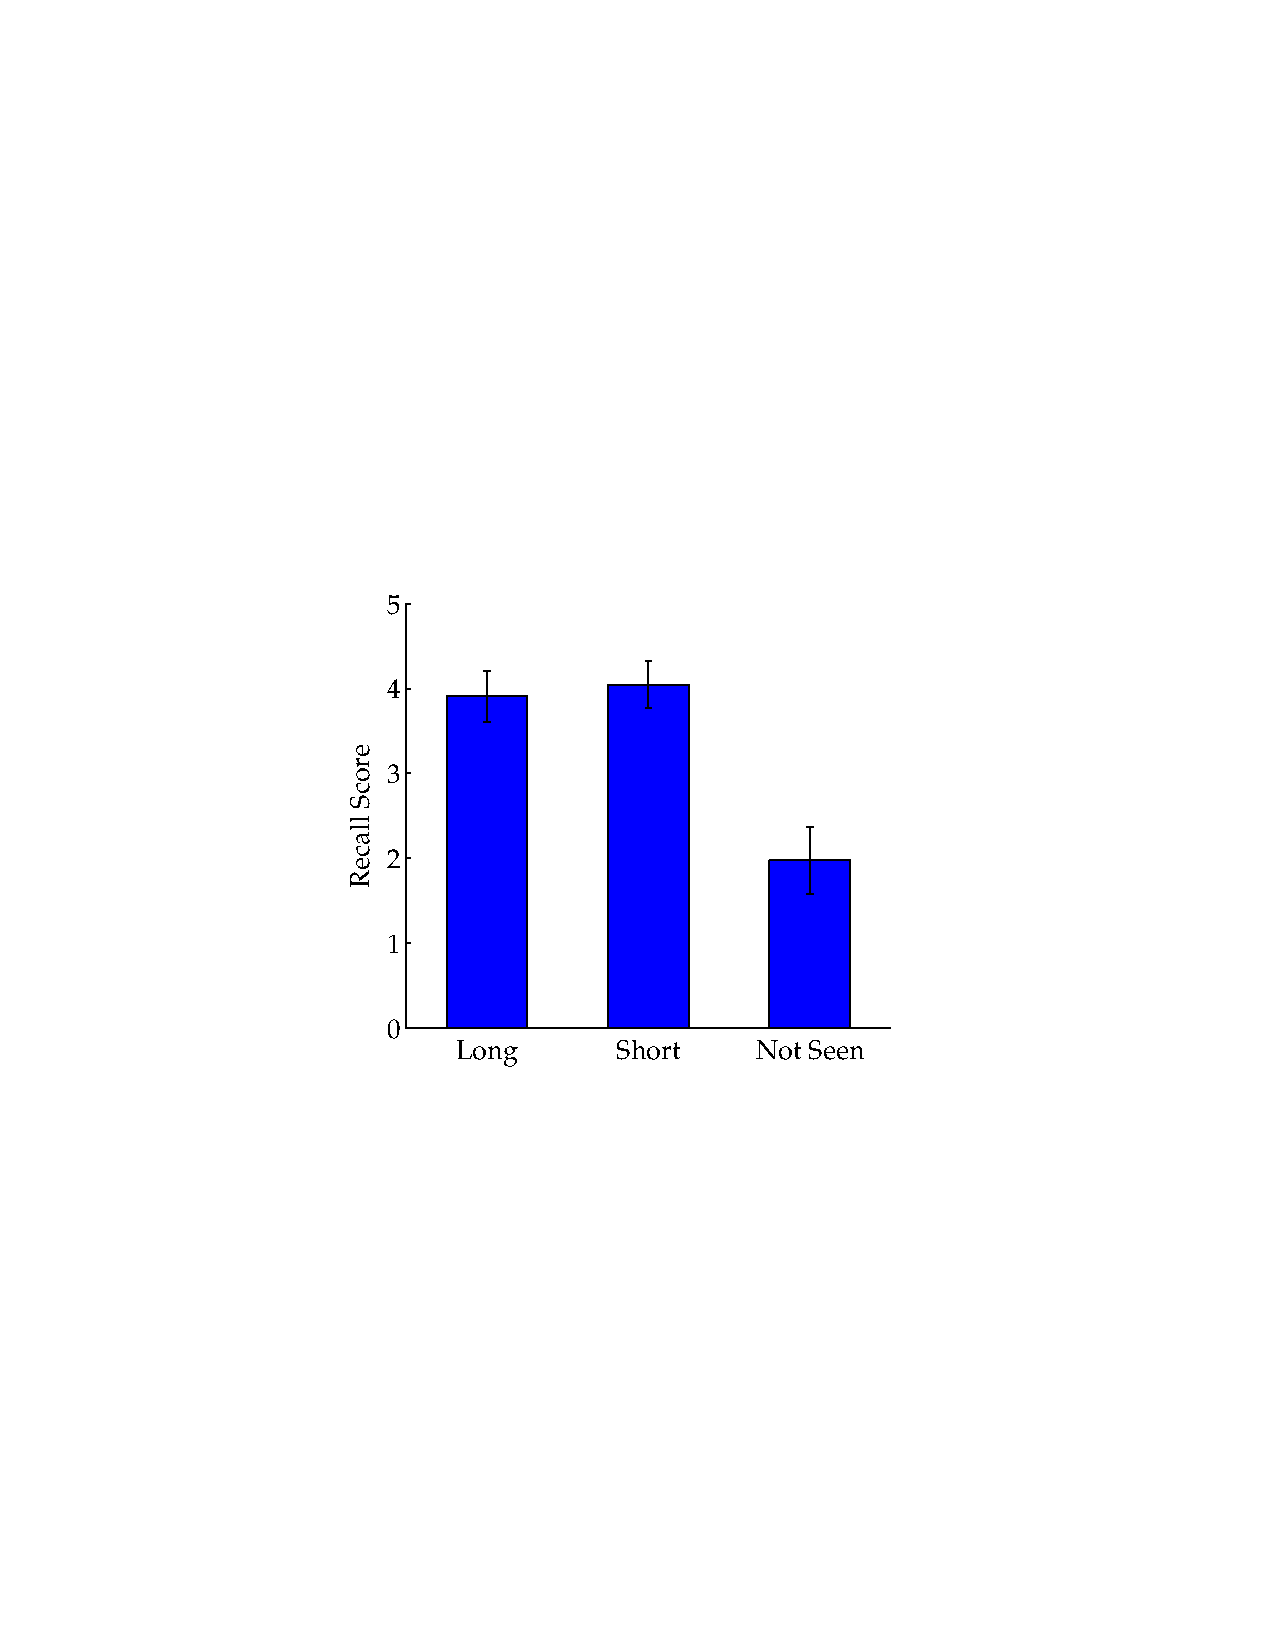
\includegraphics[width=60mm,height=54mm,trim=65mm 103mm 68mm 100mm]{./eps/memtest_leng}}
  \caption{긴 응시와 짧은 응시에 대한 장기 기억 능력 시험 결과 이다. 긴 응시와 짧은 응시에 대한 기억력 점수는 통계적으로 유의미 하지 않았다 (p $=$ 0.5051). 오차 막대는 $\pm$ 2 표준 오차를 뜻 한다. 실험에 대한 자세한 설명은 ~\nameref{subsec:experiment2} 소절을 참조한다.}
  \label{fig:memtest-leng}
\end{figure}

\begin{figure}
  \centerline{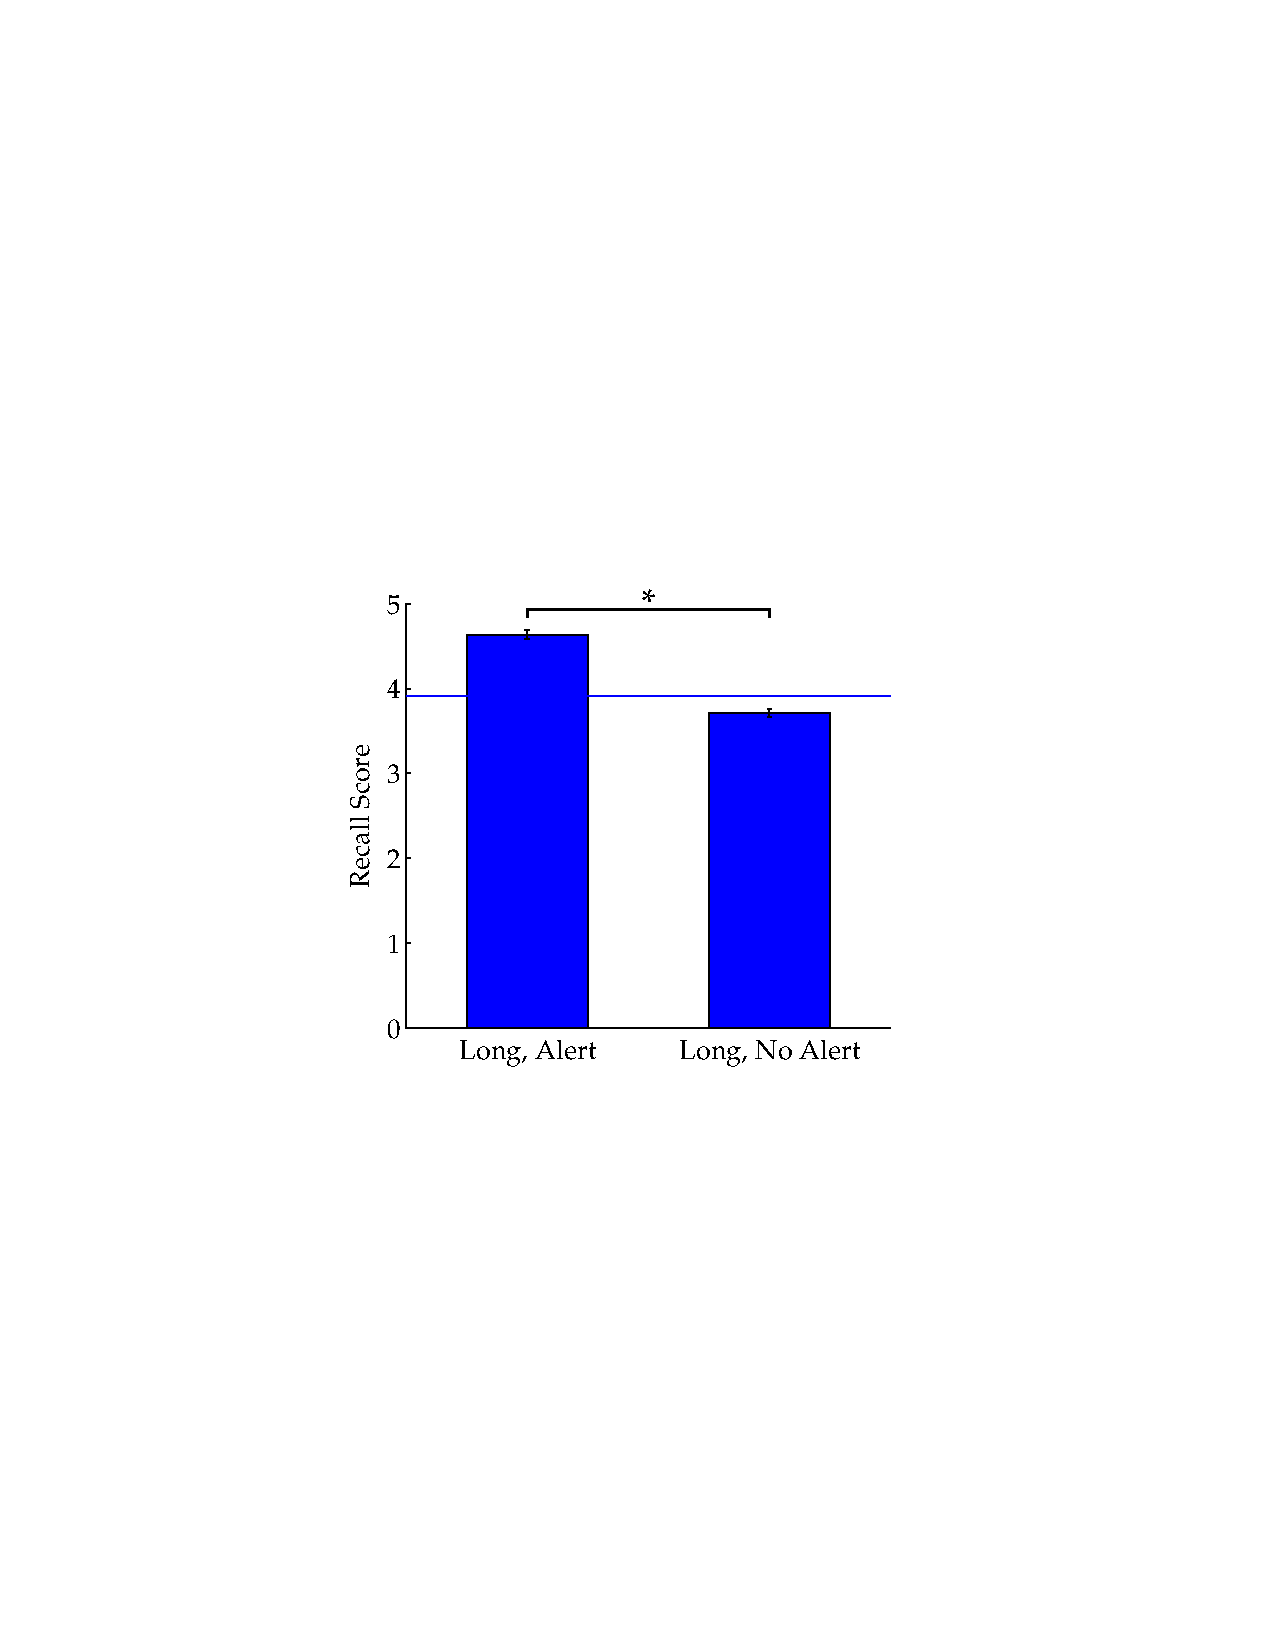
\includegraphics[width=60mm,height=54mm,trim=65mm 103mm 68mm 100mm]{./eps/memtest_long.pdf}}
  \caption{The memory test result for the \textit{long} fixation which is on the \textit{Alert} sequence or the \textit{No Alert} sequence. The number of cases from 11 participants are 19 and 69, respectively. The difference between two means is statistically significant, the p-value of two-sample t-test for the \textit{Alert} type is 0.0104 ($<$ 0.05). The blue horizontal line indicates the mean scores of the \textit{long} fixated sequences. Error bars indicate $\pm$ 2 SEMs.}
  \label{fig:memtest-long}
\end{figure}

\begin{figure}
  \centerline{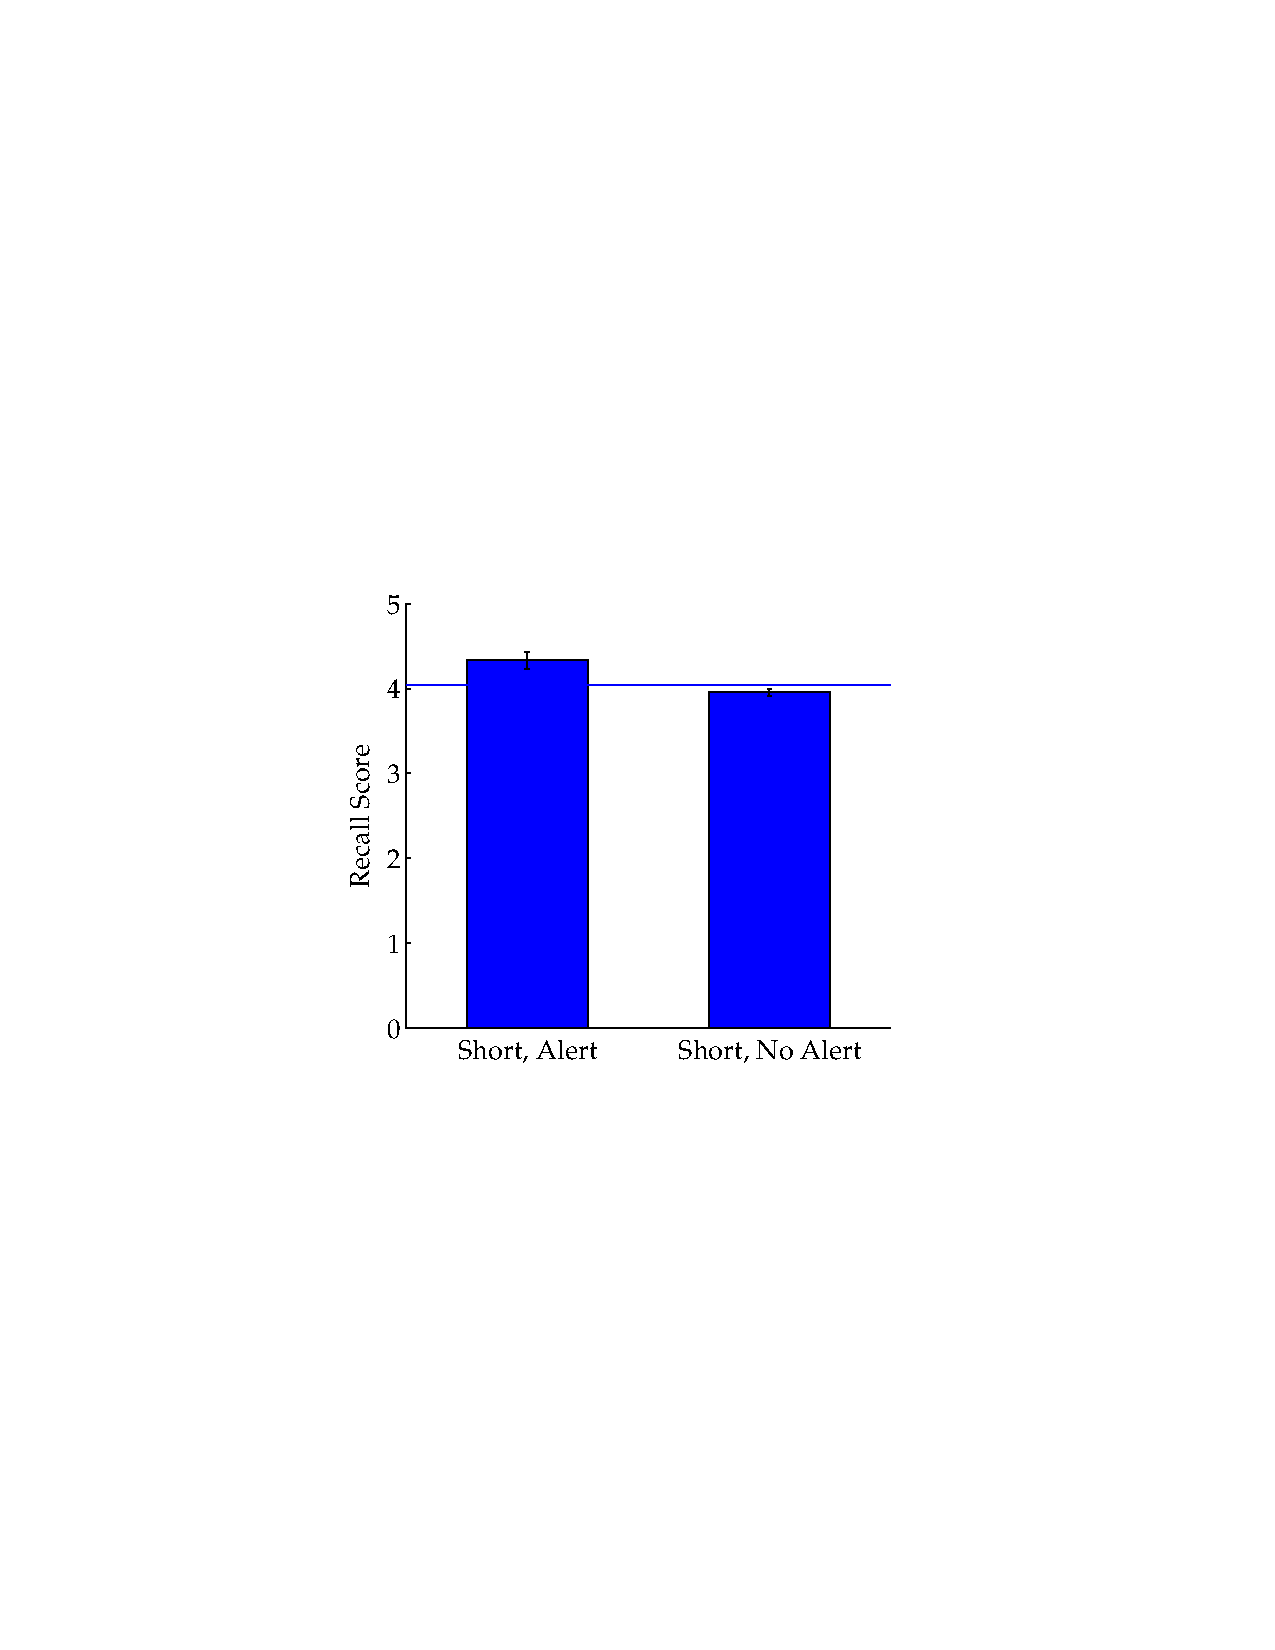
\includegraphics[width=60mm,height=54mm,trim=65mm 103mm 68mm 100mm]{./eps/memtest_short.pdf}}
  \caption{The memory test result for the \textit{short} fixation types which is on the \textit{Alert} sequence or the \textit{No Alert} sequence. The number of cases from 11 participants are 21 and 67, respectively. The p-value of two-sample t-test for the \textit{Alert} type is 0.2484 ($>$ 0.05). The blue horizontal line indicates the mean scores of the \textit{short} fixated sequences. Error bars indicate $\pm$ 2 SEMs.}
  \label{fig:memtest-short}
\end{figure}

\begin{enumerate}[itemsep=0pt,parsep=0pt]
	\renewcommand{\theenumi}{\arabic{enumi}}
	\renewcommand{\labelenumi}{\cl\theenumi}
	\item 제목(국문)
	\item 저자명(국문) * 발표자는 공동저자와 구분 처리 \\ (예) 홍길동$^{\circ}$
	\item 소속(국문)
	\item 저자 E-mail Address
	\item 제목(영문)
	\item 저자명(영문) * 발표자는 공동저자와 구분처리 \\ (예) Kildong Hong$^{\circ}$
	\item 소속(영문)
	\item 요약
	\item 본문
	\begin{itemize}[itemsep=0pt,parsep=0pt]
	  \item 장 및 절에 해당되는 번호는  아라비아 숫자로 각각 1., 1.1 등과 같이 표기
	  \item 그림의 명칭은 하단에, 표는 상단에 그림 1 및 표 1로 표기
	\end{itemize} 
	\item 참고 문헌
	\begin{itemize}[itemsep=0pt,parsep=0pt]
	  \item 본문중에 \cite{Lee:2008,Myung:2008,Lee:2010}과 같이 참고문헌 번호를 쓰고, 그 문헌을 참고 문헌란에 인용한 순서대로 기술
	  \item 기술 순서는 저자, 제목, 학술지명, 권, 호, 쪽수, 발행년도 순으로 작성.
	\end{itemize}
	\item 부록(해당사항이 있는 경우만 작성) 
\end{enumerate}



\subsection{기타}
\begin{itemize}[itemsep=0pt,parsep=0pt]
  \item 위 유의사항 3개항목을 제외한 논문작성폰트, 크기는 임의 사용가능합니다. 
  단, 논문집(Proceedings) 제작시 축소 인쇄하므로 글자크기를 9pt 이하는 사용하지 마시기 바랍니다.
  \item 논문심사는 저자와 심사위원 상호 비공개로 진행됩니다. 
  따라서, 심사용(저자정보 삭제)과 출판용(저자정보 포함)으로 나눠 제출합니다. 
  심사용은 투고시, 출판용은 심사후 지정된 수정기간중에 각 업로드 하시면 됩니다. 
\end{itemize}

\section{\LaTeX 사용 시 유용한 팁}

\LaTeX을 사용하여 논문을 작성하면 다양한 이점이 있다.
먼저 복잡한 수식을 쉽게 작성할 수 있다.
가장 큰 장점 중 하나는 bibtex을 이용해서 참고 문헌 관리를 편리하게 할 수 있다는 것이다.
이 외에도 그림이나 표의 참조를 쉽게 할 수 있다는 것 등 다양한 장점이 있다.

여기서는 \LaTeX을 이용하여 논문을 작성할 때 많이 사용되는 명령에 대한 몇 가지 예를 제시한다.
자세한 내용은 \LaTeX에 관한 다양한 메뉴얼을 참고하기 바란다.

\subsection{문서 서식 사용}
본 latex 템플릿을 사용하는 경우에는 기본적인 여백, 폰트 크기가 KCC에서 요구하는 기본 서식을 준수한다.
또한, 문서 서식(documentclass)을 지정할 때 옵션으로 {\tt preprint}를 주면 저자 정보가 제외된다.


\subsection{수식}
\begin{equation}
\label{eq:eq1}
SumOnlyPositives(\mathcal{D}) = \sum_{\forall x \in \mathcal{D} \land x > 0 }x
\end{equation}
\eqref{eq:eq1}과 같이 수식을 바로 참조할 수 있다.
\index{equation}


\subsection{알고리즘}
Algorithm \ref{alg:sum}과 같이 알고리즘을 표현할 수 있다.
\begin{algorithm}[!ht]
\label{alg:sum}
\caption[Short label]{\texttt{SumOnlyPositives}($\mathcal{D}$)}
\begin{algorithmic}[1]
\REQUIRE a set of real number $\mathcal{D}$ 
\ENSURE sum of all non-negative elements in $\mathcal{D}$ 
\STATE $O \leftarrow 0$
\FOR{\textbf{each} $x\in \mathcal{D}$ }
	\IF{$x > 0$}  
		\STATE $O \leftarrow O + x$
	\ENDIF
\ENDFOR
\RETURN $O$
\end{algorithmic}
\end{algorithm}

  
\subsection{표}
표 \ref{tab:datasets}과 같이 표를 작성할 수 있다.
\begin{table}[!ht]
\centering
\setlength{\belowcaptionskip}{5pt}
\caption{실험 데이터의 주요 통계적 수치}
\label{tab:datasets}
\begin{tabular}{@{}lrrrr@{}} 
\toprule
{\bfseries Dataset} & $|\mathcal{D}|$ & ${\rm avg}(|x|)$ & $|\mathcal{U}|$ & ${\rm avg}(|I_i|)$ \\
\midrule
LAST.FM			&134,949	&  4.8	& 47,295	& 13.8\\
LAST.FM 4G		&			& 11.2	& 44,272	& 34.3\\
DBLP			&1,298,016	&  8.6	&381,450	& 29.3\\
TREC			&348,566	& 77.1	&298,302	& 90.1\\
UKBENCH			&10,200		&425.7	&533,412	&  6.9\\
\bottomrule
\end{tabular}
\end{table}


\subsection{그림}

그림 \ref{fig:example1}과 같이 외부 그림을 삽입할 수 있다.

\begin{figure}[!ht]
\centering
\includegraphics[width=0.4\textwidth]{features.pdf}
\caption{그림 예제}
\label{fig:example1}
\end{figure}
\index{figure}


\subsection{도형 직접 그리기}

그림 \ref{fig:picture}와 같이 몇 가지 명령을 이용해서 간단한 그림을 직접 그릴 수 있다.

\begin{figure}[h!]
\centering
\setlength{\unitlength}{6pt}
\begin{picture}(40,10)
\put(20,5){\circle{6}$y$}
\put(3,2){\framebox(5,4){$x$}}
\end{picture}
\caption{간단한 도형 그리기 예제}
\label{fig:picture}
\end{figure}



\subsection{참고 문헌 관리}
각각의 참고 문헌을 bibtex 형식으로 관리하고,
다양한 형식으로 쉽게 출력할 수 있다.
bibtex에 관한 다양한 참고 문헌을 참조하기 바란다.
컴퓨터 공학 관련 분야에서는 {\em ieeetr, IEEE, unsrt, plain, abbrv}와 같은 형식이 자주 쓰인다.


\bibliographystyle{ieeetr}
\bibliography{kim2014activelong}

\end{document}
